\chapter{Implementation}
\label{ch:Implementation}
\todo[inline]{intro her må endres da deler av Julia-forklaringen er flyttet utenfor.}
In this chapter, I will discuss why it is interesting to implement AD in Julia. I will also give some implementation-specific details and benchmark the implementation against other AD libraries in Julia and MATLAB.

\section{Automatic Differentiation in Julia}
\label{sec:ADInJulia}
As discussed in \autoref{ch:Julia}, Julia seems to be the perfect language for numerical applications and it would be interesting to see how it performs compared to MATLAB.
When it comes to AD in Julia, there are already some packages that can be used. Most of them are backward AD-packages designed for machine learning, for example AutoGrad \citep{knet2016mlsys} and Zygote \citep{innes2018don}. The reason why AD-packages for machine learning are based on backward AD is that machine learning, without going to deep into the subject, largely amounts to the minimization of functions with a large number of input parameters, but with only one output parameter. As discussed in \autoref{sec:BackwardAD}, backward AD is much more efficient than forward AD in these types of evaluations. For numerical applications there is usually many input parameters and output parameters. Hence there is no clear advantage of using backward AD compared to forward AD. 

There is one package called \textit{ForwardDiff} \citep{ForwardDiff} being developed by the Julia community that uses forward AD. ForwardDiff relies on dual numbers as explained in \autoref{sec:DualNumbers} extended to multiple dimensions. This is called multidimensional dual numbers and a vector \textbf{x} of length $n$ is represented as
\begin{align*}
    \textbf{x} = \begin{bmatrix}
    x_1 + \epsilon_1 \\
    \vdots \\
    x_i + \epsilon_i \\
    \vdots \\
    x_n + \epsilon_n \\
    \end{bmatrix}.
\end{align*}
 This package works very well for some applications, but especially numerical solution of PDEs it has some limitations that are not ideal, for example: 
\begin{itemize}
    \item The function to differentiate can only accept a single argument. This is possible to work around; if you have vector function $f$ with input parameters $x,y,z \in \Re^n$, you can merge them into one vector of length $3n$ and then obtain the Jacobian. Although this works and you get the correct answer, it is not optimal as you would have to make local workarounds to make the code work, causing unreadable code.
    \item The function we want to differentiate must be on the form of a generic Julia function, such as: $g(x) = 3x*x$. Here $x*x$ symbolize element-wise multiplication. This means that if we have a function like $h(x) = 3x*x + \text{sum}(x)$, where all elements in $g(x)$ are added with the sum of all elements in $x$, it will not be possible to use \textit{ForwardDiff} to obtain the Jacobian. This limitation also prevents us from having a function that we evaluate for all points, and then add boundary conditions for some points later. This is a feature that is essential in PDE-based simulators.
    \item The Jacobian calculated by \textit{ForwardDiff} is a full matrix. In some cases the Jacobian is dense anyway, so this will not have any major adverse effects, but in many numerical applications, and particularly in numerical solution of PDEs, the Jacobian will be sparse. By representing a sparse matrix on a full matrix format, a lot of potential computation efficiency is lost.
\end{itemize}

\section{Implementation of Automatic Differentiation}
\label{sec:ImplementationAD}
When it comes to efficient implementation of AD, there are two factors to consider. Firstly, it must be easy and intuitive to use. Secondly, the code must be efficient as it will be used in computational demanding calculations. A convenient way to store the AD-variables in Julia is to make a structured array (\texttt{struct}) that has two member variables, \texttt{val} and \texttt{jac}, that store respectively the value and the corresponding Jacobian: 
\lstinputlisting{code/AD_struct.jl} 
The \texttt{val} variable is a vector with elements of type \texttt{Float64}. If the AD-variable is only a scalar, the implementation can either stick to \texttt{val} being a vector, only of length one, or it can be just a scalar in this specific case. Always representing \texttt{val} as a vector is most consistent and can avoid problems that may occur when we do not know what types the AD struct contains at different times. When it comes to the Jacobian, there are multiple ways of storing the matrix. Depending on the application, how much, and what type of manipulation of the matrix you are going to do, the choice is based on efficiency and convenience. I will describe two different methods on how to store the Jacobian. Both implementations are inspired by two different implementations in MRST \citep{lieMrstUrl}. 

\subsection{\texttt{ForwardAutoDiff} (\texttt{FAD})}
\label{sec:FAD}
In the first implementation, the Jacobian \texttt{jac} is represented as a list of subblocks. Each element in the list is a sparse matrix that represent the Jacobian w.r.t. a single primary variable. This implementation gives the freedom to easily work with the subblocks of the Jacobian that correspond to a single primary variable. Before introducing the second implementation of the Jacobian, I will continue to explain the implementation of what I have called \texttt{ForwardAutoDiff}(\texttt{FAD}), which is defined with the following struct:
\lstinputlisting{code/FADStruct.jl}


To obtain a working AD library, we need to implement operators for the \texttt{FAD} data structure. The importance of how you implement the AD operators and elementary functions can be expressed in a short example: Assume you have two \texttt{FAD} variables $x$ and $y$ and that you want to compute the function $f(x,y) = y+\exp(2xy)$. If the implementation is based on making new functions that take in \texttt{FAD}-variables as input parameters, the evaluation of $f$ will look something like this: 
\begin{center}
    $f$ = \texttt{FADplus}($y$,\texttt{FADexp}(\texttt{FADtimes}(2,\texttt{FADtimes}($x,y$)))).
\end{center}
This is clearly not a suitable way to implement AD as it quickly becomes difficult to see what type of expression it is. If you did not know what type of function f is, it would take you quite some time to figure it out. And more importantly, the possibility for human error becomes very large when you have to write unreadable code like this. This approach should be avoided. 

\cite{doi:10.1137/080743627} and \cite{lieMrstUrl} suggest a much more elegant implementation, in which one, instead of making new functions that take in \texttt{FAD}-variables as parameters, overloads the standard operators (+,-,*,/) and the elementary functions (exp, sin, log, etc.). This is where the elegance of having a custom \texttt{FAD} struct appears. In Julia, we can use \emph{multiple dispatch} to call our implementation of standard operators and elementary functions when they are used on \texttt{FAD} structs. A quick explanation of \emph{multiple dispatch} that satisfies our needs is that the compiler at run-time understands what types are given as input for either an operator or a function and chooses the correct method based on this. To demonstrate, the following function \lstinputlisting{code/overload_plus_operator_AD.jl} 
overloads the + operator. Here, we import the + operator from \texttt{Base} (which is where the standard functions in Julia lie) and overload it for \texttt{FAD} variables. For brevity, I have removed checks and edge cases and only left the method for \texttt{FAD} variables with equal length. The broadcast function adds each Jacobian for each primary variable together. This implementation of the + operator is only used when there are \texttt{FAD} variables on both sides of the operator. Hence, if $z = x+y$ is computed for $x = 1$ and $y = 3$, Julia understands that it is not the definition above, but the normal addition for integers it should use. But if $x,y = \texttt{initialize\_FAD}(1,3)$ is declared, so that $x$ and $y$ both are \texttt{FAD} variables, then Julia's multiple dispatch will understand that the new definition of the "+"-operator should be used on the expression $z = x+y$. What we need to remember is that if I now write $z = x + 3$, with $x$ as an \texttt{FAD} variable, Julia will deploy an error message. This is because we also have to implement
\lstinputlisting{code/overload_plus_operator_number.jl}
Here, the first function will be used if the + operator is used with an \texttt{FAD} variable on the left hand side and a number on the right. The last line is a compact way of writing the opposite function, which will be used when the number is the left-hand argument to the + operator. Once all such options are implemented for the four elementary algebraic operators, as well as for elementary unary functions, we can simply write $f = y+\exp(2*x*y)$ and Julia will understand that it is our implementation of + and * operators and the exponential function that shall be used. The variable $f$ will now become an \texttt{FAD}-struct with the correct value and derivatives. 

Up until now, I have only discussed implementation of \texttt{FAD} for scalar variables. But another advantage of Julia's multiple dispatch system is clear if we start looking at vector variables and functions. In some situations, like in \autoref{ch:FlowSolver}, we want to sum over all the elements in the vector. If we look at how we can overload the \texttt{sum} function, one might think that we would try something like
\lstinputlisting{code/overload_sum.jl}
which would indeed work. Nonetheless, a more elegant approach that fully exploit Julia's multiple dispatch, would be to overload the \texttt{iterate} function. This function explains how we shall iterate through an AD variable: 
\lstinputlisting{code/iterate.jl}
Now, the built-in \texttt{sum} function will work on AD variables since it knows how to iterate through the variables. When it adds up the values, the "+"-operator we defined above is being used. And not only that! All built-in functions that iterate through the input will also work (given that the functions they use on the variable also are overloaded). As an example, if we now overload the division operator as well as the ones talked about above, the Base function \texttt{mean} will also work on \texttt{FAD} variables with no extra work!

\subsection{Element-wise and Vector Multiplication}
%When one introduces AD for vectors, one needs to discuss how to handle multiplication and division.
In mathematical programming languages like MATLAB and Julia, there is a difference between the * and .* operators. The first operator, *, is regular vector multiplication, meaning if $v$ is a row vector and $u$ is a column vector, both of length $n$, then $v*u$ is the normal vector product that results in a scalar, whereas $u*v$ gives an $n\times n$ matrix in which each row in $v$ is multiplied by the corresponding row value of $u$. An attempt to evaluate $u*u$ will end in an error message saying that "the dimensions do not match matrix multiplication". 

The .* operator, on the other hand, represents element-wise multiplication. This means that if we have regular column vectors like $u$ and $w = v'$, where $w$ is the transpose of $v$, the evaluation of $u.*w$ will be element-wise multiplication of $u$ and $w$, into a new vector of the same dimensions as $u$ and $w$. Here, one needs to make a choice in the implementation of multiplication and division for AD in Julia, because as of now, there are no good ways of overloading any dot operators for custom types such as AD. \emph{\citet{JuliaIssueDot}} explains the problems of overloading the element-wise .* operator, and states that there is no good way of actually doing this. The issue has still not been resolved. With this in mind, and that there will only be used element-wise multiplication in this project, I have decided that I herein redefine * and implement it as element-wise multiplication. This means that if I have written regular multiplication expressions consisting of at least one AD-variable, element-wise multiplication will be executed.

\subsection{Optimizing \texttt{ForwardAutoDiff}}
By looking closer at the implementation of the Jacobian in \texttt{FAD}, we can find that in some cases there are better approaches to storing the Jacobian that will gain computational efficiency. Before looking closer at the specific situations, I will explain how the sparse matrix type, \texttt{SparseMatrixCSC}, that \texttt{FAD} uses is built up and how it works. \texttt{SparseMatrixCSC} stands for \textit{Compressed Sparse Column Sparse Matrix Storage} and according to Julia docs \emph{\citep{SparseMatrixCSC}} the SparseMatrixCSC struct is given as
\lstinputlisting{code/SparseMatrixCSCStruct.jl}
It represents a matrix with three vectors and two integers. The integers represent the size of the matrix and the three vectors represent all non-zero elements in the matrix. To explain how the vectors work, consider the example of a matrix \textbf{A} with the corresponding \texttt{SparseMatrixCSC} struct variables:
\begin{multicols}{2}
    \begin{align*}
        \textbf{A} = \begin{pmatrix}
        1&0&0&5&0\\
        0&3&0&6&0\\
        0&0&0&0&7\\
        2&4&0&0&0\end{pmatrix}
    \end{align*}
    \columnbreak
    \begin{align*}
        \texttt{m} &= 4\\
        \texttt{n} &= 5\\
        \texttt{colptr} &= [1, 3, 5, 5, 7, 8]\\
        \texttt{rowval} &= [1, 4, 2, 4, 1, 2, 3]\\
        \texttt{nzval} &= [1, 2, 3, 4, 5, 6, 7].
    \end{align*}
\end{multicols}
Here, \texttt{nzval} contains all the nonzero elements in \textbf{A}. The order of the numbers is given by column from left to right and then row from top to bottom. The vector \texttt{rowval} has the same ordering as \texttt{nzval} and gives the row number to the corresponding value in \texttt{nzval}. The vector \texttt{colptr} contains the information of how many non-zero numbers there are in each column. For column number $i$, the sequence \texttt{colptr}$[i]$:\texttt{colptr}$[i+1]-1$ gives the indices in \texttt{nzval} and \texttt{rowval} that correspond to values in this column. For matrix A and column number 2 we get the indices
\begin{equation*}
    \texttt{colptr}[2]:(\texttt{colptr}[3]-1) \Longrightarrow 3:4,
\end{equation*}
which gives row number 2 and 4 and values 3 and 4. For a column with only zero elements, like column 3, the sequence becomes
\begin{equation*}
    \texttt{colptr}[3]:(\texttt{colptr}[4]-1)\Longrightarrow 5:4,
\end{equation*}
which indicates that there are no nonzero elements in this column. 

This way of storing a matrix will decrease both memory usage and computational efficiency dramatically when working with large and sparse matrices compared to storing the full matrix. When performing operations on the matrix, e.g., an element-wise vector-matrix  multiplication, the computational gain comes from the opportunity to neglect all zero values. If we store the matrix as a full dense matrix, then we have to compute a lot of multiplications that ends up being zero, which we with a sparse matrix structure can avoid computing. The method, however, brings some extra work that consist of doing numerous checks to make sure that we have done the multiplication correctly. Take the example from \autoref{sec:FADWithVectorParameters}, where we wish to compute $f = 2\cdot \textbf{x}\cdot \textbf{y}$ for the primary variables $\textbf{x},\textbf{y}\in \Re^3$ defined in \eqref{def:VectorAD}. Initializing the primary variables as \texttt{FAD}-structs gives 
\begin{multicols}{2}
    \noindent
    \begin{align*}
        \textbf{x} = \left[\adpair{\begin{pmatrix}1\\2\\3
        \end{pmatrix}}{\left\{\adpair{
        \begin{pmatrix}
        1&0&0\\
        0&1&0\\
        0&0&1\end{pmatrix}}
        {\begin{pmatrix}
        0&0&0\\
        0&0&0\\
        0&0&0
        \end{pmatrix}}\right\}} \right]
    \end{align*}
    \begin{align*}
        \textbf{y} = \left[\adpair{\begin{pmatrix}4\\5\\6
        \end{pmatrix}}{\left\{\adpair{
        \begin{pmatrix}
        0&0&0\\
        0&0&0\\
        0&0&0\end{pmatrix}}
        {\begin{pmatrix}
        1&0&0\\
        0&1&0\\
        0&0&1
        \end{pmatrix}}\right\}} \right].
    \end{align*}
\end{multicols}
Here, I have written out the Jacobians as full matrices for better visualization, although in theory they will be stored as \texttt{SparseMatrixCSC} structs. In the multiplication of the two \texttt{FAD}-variables, the element-wise multiplication of the values is not interesting and we will instead focus on how we obtain the new Jacobian for $\textbf{x}\cdot \textbf{y}$. Similarly as in \autoref{sec:FADWithVectorParameters} we find the new Jacobian using the product rule, but now we can separate the operations into two calculations. First, we have the Jacobian for the primary variable \textbf{x}:
\begin{align*}
    \begin{pmatrix}
        4&0&0\\
        0&5&0\\
        0&0&6\end{pmatrix}
        \cdot
        \begin{pmatrix}
        1&0&0\\
        0&1&0\\
        0&0&1
        \end{pmatrix}
        +
        \begin{pmatrix}
        1&0&0\\
        0&2&0\\
        0&0&3
        \end{pmatrix}
        \cdot
        \begin{pmatrix}
        0&0&0\\
        0&0&0\\
        0&0&0
        \end{pmatrix}
        \Longrightarrow
        \begin{pmatrix}
        4&0&0\\
        0&5&0\\
        0&0&6
        \end{pmatrix}.
\end{align*}
Then for the primary variable \textbf{y} we obtain the Jacobian
\begin{equation}
    \label{eq:JacobianCalculationY}
    \begin{pmatrix}
        4&0&0\\
        0&5&0\\
        0&0&6\end{pmatrix}
        \cdot
        \begin{pmatrix}
        0&0&0\\
        0&0&0\\
        0&0&0
        \end{pmatrix}
        +
        \begin{pmatrix}
        1&0&0\\
        0&2&0\\
        0&0&3
        \end{pmatrix}
        \cdot
        \begin{pmatrix}
        1&0&0\\
        0&1&0\\
        0&0&1
        \end{pmatrix}
        \Longrightarrow
        \begin{pmatrix}
        1&0&0\\
        0&2&0\\
        0&0&3
        \end{pmatrix}.
\end{equation}
We immediately observe that two of the multiplications are unnecessary, since one of the matrices is a null matrix. Remember then that the left matrix in all the calculations above actually is a vector that we have transformed into a diagonal matrix to illustrate how the element-wise multiplication happens. This means that when the previous Jacobian is a diagonal matrix, what we actually can do to obtain the new Jacobian, is element-wise multiplication between the vector on the left hand side and the vector that is the diagonal on the Jacobian. And even better, when the previous Jacobian is the identity matrix, like in calculation \eqref{eq:JacobianCalculationY}, the product is simply a diagonal matrix with the left hand side vector on the diagonal. This is where the idea of optimizing \texttt{FAD} comes from. By knowing what type of Jacobian we have at all times, we can sometimes take safe shortcuts in our calculations. 

\subsection{Custom Jacobian Automatic Differentiation}
Custom Jacobian Automatic Differentiation (\texttt{CJAD}) is what I have chosen to call the optimized \texttt{FAD}. \textit{Custom Jacobian} comes from having four different types of Jacobians. The structure of \texttt{CJAD} is similar to \texttt{FAD}, but instead of storing all the Jacobians as a vector consisting of \texttt{SparseMatrixCSC}-types, each element in the vector is now of type \texttt{CustomJac}:
\lstinputlisting{code/CJAD-struct.jl}
\texttt{CustomJac} is an abstract type that has four structs that extend it:
\begin{itemize}
    \item \texttt{NullJac} -- a struct only containing two numbers that represents the number of rows and columns in a null matrix.
    \item \texttt{IdentityJac} -- a struct only containing one number that represents the number of rows and columns in an identity matrix.
    \item \texttt{DiagJac} -- a struct containing a vector called \texttt{jac} with the diagonal values of a diagonal matrix. The length of \texttt{jac} equals the number of rows and columns.
    \item \texttt{SparseJac} -- a struct containing a \texttt{SparseMatrixCSC} matrix called \texttt{jac}.
\end{itemize}
Now, the multiple dispatch system in Julia comes in handy once again. Since Julia understands at run-time what type of \texttt{CustomJac} we have -- whether it is a \texttt{NullJac}, \texttt{IdentityJac}, \texttt{DiagJac} or \texttt{SparseJac} -- we can implement different methods for all possible combinations. In each implementation, we now know what type of matrix we are dealing with, and we can thus optimize the performance. As an example, consider calculating the Jacobian w.r.t primary variable \textbf{y} in \eqref{eq:JacobianCalculationY} (All the implementations of operators on structs extending the \texttt{CustomJac} type are called from outer functions that check the legality of the operations; hence, the following code excerpts contain no safety checks.) First, we have a vector multiplied element-wise by a null matrix. The implementation
\lstinputlisting{code/vectorTimesNullJac.jl}
knows immediately that there is no need to do any calculations, the result will be a null matrix of the same size as before. Without diving too deep into the implementation of \texttt{SparseMatrixCSC}, but only by considering what kind of information the \texttt{SparseMatrixCSC}-struct contains, this implementation should not make a big difference in the computational efficiency of \texttt{CJAD} compared to \texttt{FAD}. The reason for this is that the implementation of \texttt{SparseMatrixCSC} will also quickly realize that its vectors are of length zero and the matrix is a zero matrix. The speed difference of the two implementations will hence be small for this particular operator. However, the second calculation in \eqref{eq:JacobianCalculationY} is a vector multiplied element-wise by an identity matrix. The result will be a diagonal matrix with the values of the vector on the diagonal. The \texttt{SparseMatrixCSC} implementation only knows that we have a sparse matrix with some values and is unaware that it actually is the identity matrix. This means that it has to do all the calculations without any shortcuts.  The implementation for \texttt{IdentityJac}, however, automatically knows the result of this calculation and simply makes a diagonal Jacobian with the vector on the left hand side:
\lstinputlisting{code/vectorTimesIdentityJac.jl}
This is the first calculation we have seen that will make \texttt{CJAD} considerably more computational efficient than \texttt{FAD}. To finish the calculations in \eqref{eq:JacobianCalculationY}, we finally have to add a null matrix and a diagonal matrix. Since there is really no need of doing this adding, the implementation simply returns the diagonal matrix:
\lstinputlisting{code/nullJacPlusDiagJac.jl}
For the same reason as explained for the element-wise multiplication between a vector and a \texttt{NullJac} matrix, this implementation will only have small advantages compared to the \texttt{SparseMatrixCSC} implementation used in \texttt{FAD}, which will also quickly figure out the needlessness of the calculation.

Another type of calculation that \texttt{CJAD} will do more efficient than \texttt{FAD} is when a vector is element-wise multiplied with a diagonal Jacobian. The operator that multiplies a vector times an \texttt{CJAD}-variable is often used, not only in itself, but also because it appears every time a chain or product rule is used. The product rule is used every time we multiply two \texttt{CJAD}-variables, and the chain rule appears when we evaluate an elementary function like $\exp$ or $\sin$ or if we evaluate an exponential of a \texttt{CJAD}-variable. If the Jacobian is of type \texttt{DiagJac}, the corresponding element-wise multiplication is simply two diagonal matrices multiplied together. \texttt{CJAD}'s implementation knows this and can multiply the two vectors element-wise and obtain the new diagonal of the new Jacobian:
\lstinputlisting{code/vectorTimesDiagJac.jl}
The same operation for \texttt{FAD} will be slower since \texttt{SparseMatrixCSC} does not possess any information that the matrix is diagonal and thus has to perform the operation as a regular multiplication between to sparse matrices. This will include checks to be certain that the multiplication is done correctly, and will hence be slower than multiplying two vectors element-wise. As said, this operation appears often, since it is used in the chain rule and in the product rule. Consider the product rule and the implementation
\lstinputlisting{code/productRule.jl}
We loop through all the Jacobians and perform the product rule to obtain the new Jacobians.  Here, \texttt{A.val} and \texttt{B.val} are the value vectors, whereas \texttt{B.customJacs[i]} and \texttt{A.customJacs[i]} are any of the four extensions of \texttt{CustomJac}. In every iteration in which at least one of the Jacobians is a special case and not the general\texttt{SparseJac}, we will gain computational efficiency like explained for the element-wise multiplication operator between a vector and a \texttt{NullJac/IdentityJac/DiagJac}. If both the Jacobians are different from \texttt{SparseJac}, we also gain computational efficiency from the addition operator. Just like for the element-wise multiplication, element-wise addition is faster for \texttt{NullJac/IdentityJac/DiagJac} than it is for the sparse matrices in \texttt{SparseMatrixCSC}.

When both Jacobians are general sparse matrices, \texttt{CJAD} and \texttt{FAD} are equal because \texttt{CJAD} transitions to use the \texttt{SparseMatrixCSC}-library as well with its \texttt{SparseJac} type. Let us now therefore look closer into how we handle the overloading of element-wise multiplication for \texttt{SparseJac}.  There are at least two different ways of implementing this operator that will use different parts of the \texttt{SparseMatrixCSC} library. The first possibility is to convert the vector into a sparse diagonal matrix and perform a matrix--matrix multiplication with \texttt{SparseMatrixCSC} matrices:
\lstinputlisting{code/vectorAsMatrixTimesSparseJac.jl}
I will call this method the \textit{matrix-multiplication} method. The second method keeps the vector form and uses element-wise multiplication between the vector and the \texttt{SparseMatrixCSC} matrix:
\lstinputlisting{code/vectorTimesSparseJac.jl}
I will call this the \textit{dot-multiplication} method. As it is difficult to say without first-hand knowledge of the implementation of \texttt{SparseMatrixCSC} which method is best to implement, I will test the two methods against each other. 
\todo{Klarte ikke å finne grunnen til dette ved å se i kildekode. Kanskje noen på SINTEF vet hvorfor?}
To this end, I have created a random vector of length 40 and a random sparse matrix of size $40\times 40$ having 20 percent nonzero elements. I then perform the element-wise multiplication 10 000 times to separate the efficiency of the two methods. To check which method is actually more efficient, and by how much, we can use the \textit{@btime} macro function from the \emph{\cite{BenchmarkTools}} library. This function gives us the number of allocations, the amount of memory used, and the time spent.
\autoref{tab:VectorMatrixMultiplicationSmallMatrix} reports the results\footnote{All benchmarks in this project are performed on a MacBook Pro (Retina, 13-inch, Late 2013), 2,8 GHz Intel Core i7 processor and 16 GB 1600 MHz DDR3 memory.} of this test.
\begin{table}[H]
    \centering
    \caption{The number of allocations, amount of memory, and time spent for element-wise multiplication of a vector of length 40 and a sparse matrix of size $40\times 40$ with 20 percent nonzero elements. The vector and matrix are multiplied together 10 000 times.}
    \label{tab:VectorMatrixMultiplicationSmallMatrix}
    \def\arraystretch{1.5}
    \begin{tabular}{cccc}
    \textbf{Method} & \textbf{Number of Allocations} & \textbf{Megabytes} & \textbf{Milliseconds} \\
        \hline
         \textit{Matrix-multiplication} & 1 420 000 & 194 & 187 \\  
         \textit{Dot-multiplication} & 60 000 & 264 & 87\\ 
         \hline
    \end{tabular}
\end{table}
The test is unequivocal:  the \textit{dot-multiplication} method has far less allocations, is more than twice as fast, but it uses a bit more memory. Based on this it might tempting to say that the \textit{dot-multiplication} method is a better choice. However, in numerical solution of PDEs, the matrices we work with are generally be much larger and very sparse. \autoref{tab:VectorMatrixMultiplicationFlowSolverMatrix} reports results for a more representative test example, in which I have used a matrix from \autoref{ch:FlowSolver}, which is of size $8000\times 8000$ and only contains 0.08 percent nonzero elements.
\begin{table}[H]
    \centering
    \caption{The number of allocations, amount of memory, and time spent for element-wise multiplication of a vector of length 8000 and a matrix of size $8000\times 8000$ with 0.08 percent nonzero elements. The matrix is taken from \autoref{ch:FlowSolver}.}
    \label{tab:VectorMatrixMultiplicationFlowSolverMatrix}
    \def\arraystretch{1.5}
    \begin{tabular}{cccc}
    \textbf{Method} & \textbf{Number of Allocations} & \textbf{Megabytes} & \textbf{Milliseconds} \\
        \hline
         \textit{Matrix-multiplication} & 240 370 & 32 & 28 \\  
         \textit{Dot-multiplication} & 180 & 10 243 & 2 458\\ 
         \hline
    \end{tabular}
\end{table}
The dot-multiplication method still requires far less allocations, but now consumes a lot more memory than the \textit{matrix-multiplication} method. As a consequence, it is almost 100 times slower than the matrix-multiplication method! This shows that for the purpose of this project, the matrix-multiplication method is a much better choice of implementation.


\subsection{Efficient Versus Readable and Elegant Code}
There is usually a fine balance between writing efficient and readable/elegant code. Sometimes you have the opportunity to do both, but often you have to choose which of them you want to give most focus. At the end of \autoref{sec:FAD}, I explained how we can elegantly implement the \texttt{sum} function, and all other built-in functions that iterate through the \texttt{FAD}-variables, only by implementing the \texttt{iterate} function. This is a very elegant use of Julia's multiple dispatch system, as we get a lot of functionality "for free". The downside, however, is that we loose potential computational efficiency that we could achieve by implementing the \texttt{sum} function ourselves. Let us define a random function $\psi$, where the AD-representation and the \texttt{sum} of $\psi$ are given by
\begin{multicols}{2}
    \noindent
    \begin{align*}
        \textbf{$\psi$} = \left[\adpair{\begin{pmatrix}1\\2\\3
        \end{pmatrix}}{\left\{\adpair{
        \begin{pmatrix}
        3&0&1\\
        2&1&0\\
        0&0&8\end{pmatrix}}
        {
        \begin{pmatrix}
        1&0&0\\
        0&1&0\\
        0&0&1\end{pmatrix}}\right\}}
        \right]
    \end{align*}
    \begin{align*}
    \\
        \texttt{sum}(\textbf{$\psi$}) = \left[\adpair{6}{
        \left\{\adpair{
        \begin{pmatrix}
        5&1&9\\
        \end{pmatrix}}{
        \begin{pmatrix}
        1&1&1\\
        \end{pmatrix}}\right\}}
        \right].
    \end{align*}
\end{multicols}
Consider now the previous approach, in which we only implemented the \texttt{iterate} function and reused \texttt{Base.sum} (i.e., the standard \texttt{sum} function in Julia) to sum the values in $\psi$. For each iterated addition, we access row $i$ in $\psi$ and add it to the total sum. This consist of extracting row $i$ from the value vector and from each Jacobian, and then creating a new AD-variable that only consists of row $i$. This leads to a lot of extra memory allocation, and in the case for $\psi$, we have to allocate memory for three new AD-variables. This extra allocation can be avoided by doing the summation of each column at once, instead of operate on a row to row basis. For \texttt{CJAD}, this can be done with the following overloaded implementation of \texttt{sum}:
\lstinputlisting{code/sum.jl}
Instead of retrieving each row, one by one, like we did using \texttt{Base.sum}, we now add up each column in one go. Here, \texttt{sum(A.val)} is the built-in sum function in \texttt{Base} for summation of a vector, and \texttt{colSum} is a function implemented in each extended type of \texttt{CustomJac}. This function sums up all the columns in the Jacobians and returns a $1\times n$ matrix. Here, $n$ is a number that depends on the dimension of the relevant primary variable ($n_\psi = 3$). In the three special cases, the function simply returns a $1\times n$ null matrix for \texttt{NullJac}, a $1\times n$ matrix containing only ones for \texttt{IdentityJac}, and a $1\times n$ matrix, which is the transposed of the diagonal vector, for \texttt{DiagJac}.  For \texttt{SparseJac}, it returns a $1\times n$ matrix in which all the nonzero values in each column are added together. To check that this new \texttt{sum} function actually is more efficient, we can again use the \textit{@btime} macro function from the \emph{\cite{BenchmarkTools}} library. By creating a random \texttt{CJAD}-variable of length 400 with all of the four different Jacobian types (all $400\times 400$ with random values), we can compare how efficient the two methods sum up the \texttt{CJAD}-variable. \autoref{tab:differentSumFunctions} reports the  result and shows that even though only implementing the \texttt{iterate} function is an elegant solution, it is much more efficient both in terms of memory consumption and runtime to implement the \texttt{sum} function specifically.

\begin{table}[H]
    \centering
    \caption{Table with the number of allocations, memory usage, and runtime spent by summing a random \texttt{CJAD}-variable of length 400 with two different summation methods.}
    \label{tab:differentSumFunctions}
    \def\arraystretch{1.5}
    \begin{tabular}{cccc}
    \textbf{Function} & \textbf{Number of Allocations} & \textbf{Kilobytes} & \textbf{Microseconds} \\
        \hline
         \texttt{sum} & 40 & 79 & 81 \\  
         \texttt{Base.sum} & 28371 & 19 597 & 58 051\\ 
         \hline
    \end{tabular}
\end{table}

\subsubsection{Vectorized and Devectorized Code}
The second issue I want to discuss is vectorized and devectorized code. The difference between the two can be quickly explained by an example. Consider two vectors \textbf{x} and \textbf{y} of the same length. To multiply the elements of the two vectors we can either use the vectorized method, \texttt{z = x .* y}, or we can loop through the vectors in the devectorized method:
\lstinputlisting{code/devectorizedExample.jl}
In a blog post, former Julia developer John Myles White explains how Julia is faster at executing devectorized code compared to vectorized code \citep{Vectorization}. This is in sharp contrast to other high-level mathematical programming languages like MATLAB, in which conventional wisdom would tell you that you have to vectorize your code to get the best computational performance. When you vectorize, MATLAB uses optimized code in C to execute the calculations. If you devectorize your code by calling a \texttt{for}-loop, you potentially bring in a lot of extra overhead. Recent development of MATLAB's just-in-time (JIT) compiler has changed the landscape a bit, and devectorized code can sometimes be significantly faster than vectorized code, in particular if the latter has to allocate a lot of temporary memory. 

In Julia, \texttt{for}-loop are generally close to matching C's speed. So you might say that "why not devectorize all the code?" And that could indeed be done, but here we have another example of the conflict between efficient and readable code. From the example with element-wise multiplication of the two vectors, the vectorized form is much more compact and readable, but according to White, the devectorized version is faster. To make a decision whether to implement vectorized or devectorized, we need to know more specifically what the differences are. White's blog post is from 2013, and since then, the vectorization in Julia has improved. Steven G. Johnson has written a newer blog post from 2017 \emph{\citep{MoreDotsJuliaBlog}}, in which he closer explains the reason why it is difficult to obtain the same speed for vectorized code as we have for devectorized code in a language like Julia. To explain this, consider two different vector functions $f$ and $g$ that we want to multiply element-wise
\begin{equation*}
    h(x,y) = f(x) \cdot g(y), \hspace{3em} f(x) = \exp(x), \hspace{3em} g(y) = \log(y).
\end{equation*}
%This example is for explaining purposes only and the functions are not meant to have any applied meaning. Since $f$ and $g$ are vector functions, $x$ and $y$ are vectors and we want to take the exponential and the logarithm element-wise to these vectors. 
In Julia, there are now three ways of obtaining $h(x,y)$. First we have the devectorized version 
\lstinputlisting{code/devectorizedFunctionEx.jl}
According to White, this should be the fastest way of obtaining $h(x,y)$. Secondly, we have the method of vectorizing the functions $f$ and $g$ such that we can call the functions with vectors and they will be performed element-wise to the input variables. I have called this method \texttt{dotsInside}:
\lstinputlisting{code/dotsInsideEx.jl}
Lastly, we do not vectorize the functions $f$ and $g$, but when we call them with the vectors $x$ and $y$, we use the dot operators on the functions to tell the Julia compiler that the functions should be executed element-wise on the input parameters. I have called this method \texttt{dotsOutside}:
\lstinputlisting{code/dotsOutsideEx.jl}
To separate the three methods, I have calculated $h(x,y)$ 1000 times for random $x$ and $y$ vectors of length 100 000 and evaluated the performance using \textit{@btime}. \autoref{tab:dotOperator} reports the results.

\begin{table}[H]
    \centering
    \caption{Table  with  the  number  of  allocations,  memory  usage,  and  runtime  spent  by  evaluating $h(x,y) = \exp(x)\cdot\log(y)$ $1\hspace{0.2em}000$ times for three different methods; $x$ and $y$ are random vectors of length $100\hspace{0.2em}000$.}
    \label{tab:dotOperator}
    \def\arraystretch{1.5}
    \begin{tabular}{cccc}
    \textbf{Method} & \textbf{Number of Allocations} & \textbf{Megabytes} & \textbf{Seconds} \\
        \hline
         \texttt{devectorized} & 2000 & 789 & 2.104 \\
         \texttt{dotsInside} & 6000 & 2 405 & 2.704 \\ 
         \texttt{dotsOutside} & 2000 & 789 & 2.121 \\  
         \hline
    \end{tabular}
\end{table}
The \texttt{devectorized} and the \texttt{dotsOutside} methods perform  identically, whereas \texttt{dotsInside} requires three times the number of allocations and memory and is also somewhat slower than the two other methods. This result confirms what Steven G. Johnson explains in \emph{\cite{MoreDotsJuliaBlog}}, where he says that the problem with vectorized operations is that they can generate new temporary arrays for each operation and that every operation is executed in a separate loop. This means that when Julia compiles the program and translates the vectorized code into devectorized code, it will compute the \texttt{dotsInside} method similar to the following code:
\lstinputlisting{code/vectorizedOperation.jl}
The compiler does this because it does not understand that all the operations are element-wise. As a consequence, it has to allocate three new arrays compared to the single new array in the \texttt{devectorized} method. However, with the \texttt{dotsOutside} method, the compiler understands that all the operations in the expression are vectorized operations and we get what Johnson calls \textit{loop fusion}. This essentially means that Julia devectorize the \texttt{dotsOutside} method into the \texttt{devectorized} method, and since Julia does not call low-level code like C to perform its vectorized code, the performance of \texttt{devectorized} and \texttt{dotsOutside} will be similar. Another advantage of using the dot operator like in \texttt{dotsOutside} is that we do not have to define if a function is vectorized or not. In other words, $f$ and $g$ can be used as functions for vectors and scalars, we specify what type of use we want when we call the function. This leads to more readable code, as we do not have to check whether a function is written for vectorization or not.

So what are the consequences for the implementation of \texttt{CJAD}? The result from \autoref{tab:dotOperator} implies that as long as we write all our vectorized code like the \texttt{dotsOutside} method or in such a manner that it is obvious for the compiler that it is only vectorized operations involved, we will have the same computational efficiency as for devectorized code. More specifically for the \texttt{CJAD} implementation, we often have a vector that is added/subtracted/divided/multiplied with another vector, and then the vectorized implementation will have the same computational efficiency as the devectorized. Since devectorized code is less readable,  implementations reported in the following will consist of vectorized code for readability.

\section{Benchmarking Automatic Differentiation}
As mentioned in \autoref{sec:ADInJulia}, Julia already has an AD library called \texttt{ForwardDiff} \citep{ForwardDiff} that uses forward AD. Hence, it would be interesting to see how the different implementations compare as the functions evaluated increase in complexity. In addition to \texttt{ForwardDiff}, I have added two AD implementation from the MATLAB Reservoir Simulation Toolbox (MRST) \citep{mrstHomepage} to the benchmark, to see how the Julia implementations compare to optimized AD tools in MATLAB. The basic implementation in MRST is similar to \texttt{FAD}, where the Jacobians has a sparse matrix structure, and is henceforth referred to as \texttt{MRST}. The second MATLAB implementation is similar to \texttt{CJAD} in the sense that it exploits the diagonal structure of some Jacobians. This method is called \texttt{MRST\_diagonal}. To benchmark the efficiency of the different AD tools, I have evaluated the vector function $f: \Re^{n\times 3} \rightarrow \Re^n $, where
\begin{equation}
\label{eq:benchmarkFunction}
f(x,y,z)  = \exp(2xy) - 4xz^2 + 13x - 7, \qquad x,y,z \in \Re^n.
\end{equation}
\autoref{fig:benchmarkADVectorFunction} reports how computational time\footnote{The benchmarks in Julia are still performed by using the benchmarking library \emph{\cite{BenchmarkTools}}. For benchmarking time in MATLAB I have taken the median of multiple tests using the stopwatch \emph{\cite{TicToc}}.} for calculating the function value and the Jacobian of the function scales as the length of the vectors $n$ increases for the different methods.

\begin{figure}[H]
    \centering
    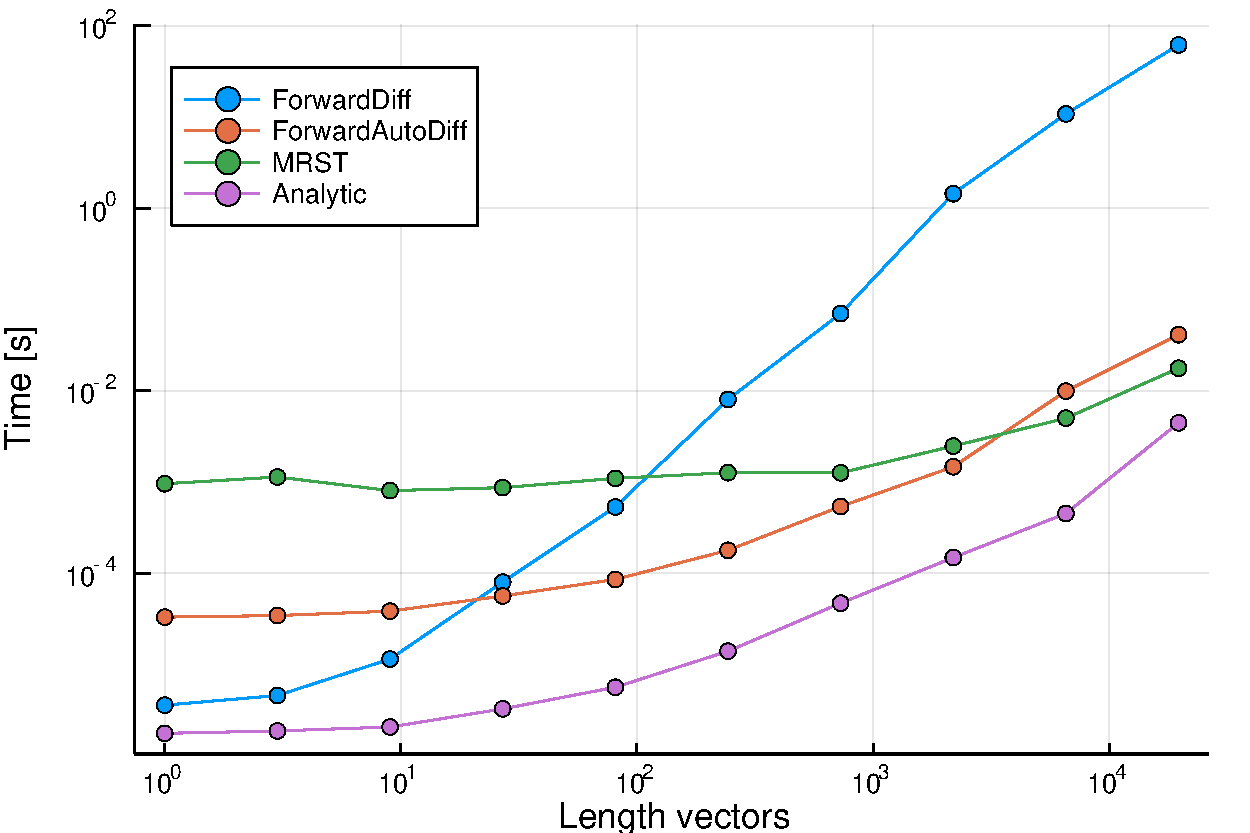
\includegraphics[width = 0.9\textwidth]{figures/benchmark_all_ADs.pdf}
    \caption{Computational time for different methods calculating the value and Jacobian of $f$ in \myeqref{eq:benchmarkFunction} as a function of length of the input vectors.}
    \label{fig:benchmarkADVectorFunction}
\end{figure}
\autoref{fig:benchmarkADVectorFunction} reports six different graphs. The first thing you observe is that \texttt{ForwardDiff} scales very badly as n becomes large. This is because it creates and works with the full $3n \times 3n$ Jacobian matrix as discussed in \autoref{sec:ADInJulia}. I stopped the benchmark of \texttt{ForwardDiff} for $n = 3^8$, as the Jacobian at this point already has more than 380 million elements. We can nevertheless observe that for small vectors, the methods implemented in MATLAB, as well as \texttt{FAD} and \texttt{CJAD}, have more overhead than \texttt{ForwardDiff} and the analytic solution. This makes them slower for small $n$, but as $n$ grows, this overhead becomes quickly negligible. Based on \autoref{fig:benchmarkADVectorFunction}, from a numerical simulation point of view, \texttt{ForwardDiff} is useless for obtaining the Jacobian of functions, as it scales badly for increasing $n$.

Apart from the conclusion on \texttt{ForwardDiff}, we can observe that it is a change in dominance at $n = 3^7 = 2187$. For shorter vectors, both methods implemented in Julia are more efficient than the two methods in MATLAB. For $n>2187$ \texttt{FAD} is the slowest, followed by \texttt{MRST}. Hence, as $n$ becomes larger than 2187, the methods in Julia and MATLAB that exploit the diagonal structure of the Jacobian perform better than the ones that only use a sparse matrix structure. This makes sense, as the evaluation of $f$ will only give a diagonal Jacobian. As $n$ becomes large, \texttt{CJAD} and \texttt{MRST\_diagonal} perform very similarly and their computational costs approach that of the analytic evaluation. What is also interesting to see is that whereas \texttt{CJAD} always is faster than \texttt{FAD}, \texttt{MRST\_diagonal} is less efficient than \texttt{MRST} for short vectors. Assuming that both the MRST implementations are optimized, this indicates that the elegant way of implementing a custom Jacobian in Julia using multiple dispatch adds very little overhead compared to MATLAB. 

The test case just discussed is highly idealized: because each element $f[i]$ of $f$ does not depend on $x[k]$, $y[k]$ and $z[k]$ for $k\not=i$, the Jacobians will keep a diagonal structure for $f$. This means that \texttt{CJAD} never uses its \texttt{SparseJac} type and that \texttt{MRST\_diagonal} can use its optimized implementation for diagonal Jacobians. If we, for example, want to calculate something like
\begin{equation*}
g(x) = \frac{x\left[2:\text{end}\right] - x\left[1:\text{end}-1\right]}{\texttt{sum(}x\texttt{)}},
\end{equation*}
the diagonal structure of the Jacobians is gone, and \texttt{MRST\_diagonal} transitions to use the \texttt{MRST} implementation, and \texttt{CJAD} has to use the \texttt{SparseJac} type, which is similar to the method used in \texttt{FAD}. This does not imply that the optimized methods are implemented in vain, since functions evaluated in numerical applications often have parts that will have diagonal Jacobians, and other parts that will not. We can thus expect to gain computational efficiency from parts of the function evaluations using \texttt{CJAD} and \texttt{MRST\_diagonal}. To assess how much we can gain, we have to look at more realistic examples. I will do this in the following \autoref{ch:FlowSolver}. 

